
% InteriorPoint_QP_beamer.tex
% 4-slide Beamer presentation explaining interior-point techniques for a convex quadratic program.
% Save as InteriorPoint_QP_beamer.tex and compile with pdflatex (or lualatex/xelatex).



% Slide 1: Problem statement + KKT
\begin{frame}{A Primer on IPM for convex QP}
  \begin{block}{Convex QP}
Consider the convex quadratic program in standard form:
\begin{align*}
  &\min_{x\in\mathbb{R}^n} \; f(x) := \tfrac{1}{2}x^T Q x + c^T x\\
  &\text{subject to }\; A x = b, \quad x \ge 0,
\end{align*}
where $Q\succeq 0$, $A\in\mathbb{R}^{m\times n}$.
\end{block}
\begin{block}{First-order (KKT) conditions}
First-order (KKT) conditions (existence of multipliers $y,z$):
\begin{align*}
  Qx + c + A^T y - z &= 0 \quad (\text{stationarity})\\
  Ax - b &= 0 \quad (\text{primal feasibility})\\
  X Z e &= 0,\quad x\ge0,\ z\ge0 \quad(\text{complementarity})
\end{align*}
where $X=\mathrm{diag}(x)$, $Z=\mathrm{diag}(z)$, $e$ is the vector of ones.
\end{block}


\end{frame}

% Slide 2: Barrier method + Newton step + figure
\begin{frame}{A Primer on IPM for convex QP}
  
\only<1>
{
  \begin{block}{Interior-point idea}
   Enforce strict positivity $x>0, z>0$ and drive $XZe=\mu e$ to zero along the \emph{central path} as $\mu\downarrow0$.
\end{block}
  \begin{block}{Barrier formulation and Newton steps}
  Use a logarithmic barrier to keep $x>0$:
\[
  \phi_\mu(x)=\tfrac{1}{2}x^T Q x + c^T x - \mu \sum_{i=1}^n \log x_i
\]
with equality constraints $Ax=b$. For fixed $\mu>0$ solve
\[\min_{x>0}\; \phi_\mu(x) \quad\text{s.t. } Ax=b.\]
\end{block}
The perturbed KKT conditions for $\mu>0$ are:
\begin{align*}
  Qx + c + A^T y - z &= 0, \\
  Ax - b &= 0, \\
  XZe &= \mu e.
\end{align*}
}
\only<2>{
We linearize these equations at $(x,y,z)$ to get the Newton system for $(\Delta x, \Delta y, \Delta z)$:
\[
  \begin{bmatrix}
    Q & A^T & -I \\
    A & 0   & 0   \\
    Z & 0   & X
  \end{bmatrix}
  \begin{bmatrix}
    \Delta x \\
    \Delta y \\
    \Delta z
  \end{bmatrix}
  = -\begin{bmatrix}
    r_d \\
    r_p \\
    r_c
  \end{bmatrix},
\]
where
\begin{align*}
  r_d &= Qx + c + A^T y - z,\\
  r_p &= Ax - b,\\
  r_c &= XZe - \mu e.
\end{align*}
This 3-block structure is the foundation of primal--dual interior-point methods.
Take a damped Newton step and project back to positive orthant with step-length chosen to maintain $x>0$.
}
% \only<2>
% {
% \vspace{2mm}
% \textbf{Figure: feasible region (linear constraints) and central path for a QP}
% \begin{center}
% \begin{tikzpicture}[scale=1]
%   % feasible polytope (two inequality lines) + ellipse objective contours
%   \filldraw[fill=gray!8] (0.3,0.4) -- (3.2,0.2) -- (3.7,2.8) -- (0.6,2.6) -- cycle;
%   % axes
%   \draw[->] (0,0) -- (4,0) node[right] {$x_1$};
%   \draw[->] (0,0) -- (0,3) node[above] {$x_2$};
%   % objective contours (ellipses)
%   \draw (1.8,1.4) ellipse (1.6 and 0.8);
%   \draw (1.8,1.4) ellipse (1.2 and 0.6);
%   \draw (1.8,1.4) ellipse (0.8 and 0.35);
%   % central path curve
%   \draw[thick,->,red] plot [smooth,domain=0:1] ( {0.5+3*\x^1.2}, {2.5-1.6*\x^0.9} ) node[right]{central path};
%   % current iterates
%   \foreach \t in {0.12,0.28,0.46,0.7,0.9}{\filldraw[black] ({0.5+3*\t^1.2},{2.5-1.6*\t^0.9}) circle (1.8pt);}
%   % optimum
%   \filldraw[blue] (1.8,1.4) circle (2.4pt) node[right] {optimal $x^*$};
% \end{tikzpicture}

% \end{center}
%}
\end{frame}



% Slide 3: Central path illustration
\begin{frame}{Illustration of the central path}
\textbf{Definition:} The \emph{central path} is the trajectory of strictly feasible points $(x(\mu), y(\mu), z(\mu))$ satisfying
\[
Qx(\mu) + c + A^T y(\mu) - z(\mu) = 0, \quad Ax(\mu) = b, \quad X(\mu) Z(\mu)e = \mu e,\; \mu>0.
\]
As $\mu \to 0$, the path converges to the optimal solution $(x^*,y^*,z^*)$.

\vspace{2mm}
\textbf{Geometric intuition:}
\begin{itemize}
  \item Each $\mu$ defines a barrier problem that smooths the feasible region.
  \item The central path traces the minimizers of these smoothed problems.
  \item Interior-point methods ``follow/approximate'' this path using Newton directions.
\end{itemize}

% \vspace{2mm}
% \begin{center}
% \begin{tikzpicture}[scale=1]
%   % axes
%   \draw[->] (0,0) -- (4.5,0) node[right] {$x_1$};
%   \draw[->] (0,0) -- (0,3.2) node[above] {$x_2$};
%   % feasible region (wedge)
%   \draw[fill=gray!10] (0.5,0.5) -- (4,0.5) -- (4,2.5) -- (0.5,2.5) -- cycle;
%   \node at (3.4,2.7) {feasible region};
%   % objective contours (ellipses)
%   \draw (2,1.4) ellipse (1.6 and 0.8);
%   \draw (2,1.4) ellipse (1.2 and 0.6);
%   \draw (2,1.4) ellipse (0.8 and 0.35);
%   % central path (smooth curve)
%   \draw[thick,red,->] plot [smooth,domain=0:1] ( {0.6+2.8*\x^1.2}, {2.4-1.7*\x^0.9} );
%   % arrows and labels for mu values
%   \foreach \m/\t in {1.0/0.1,0.3/0.4,0.1/0.7,0.03/0.9}{
%     \filldraw[red] ({0.6+2.8*\t^1.2},{2.4-1.7*\t^0.9}) circle (1.5pt);
%     \node[anchor=west,scale=0.8] at ({0.6+2.8*\t^1.2+0.1},{2.4-1.7*\t^0.9}) {$\mu=\m$};}
%   % optimal point
%   \filldraw[blue] (2,1.4) circle (2pt) node[right] {$x^*$};
% \end{tikzpicture}
% \end{center}

\vspace{1mm}
\textbf{Interpretation:} As $\mu$ decreases, the minimizer moves smoothly along the red curve toward the boundary optimum.
\end{frame}

% Slide: Central path in the positive orthant (as in Nocedal & Wright)
\begin{frame}{Central path in the positive orthant (boundary optimum)}
The central path for a problem with $x \ge 0$ approaches the boundary smoothly
as $\mu \to 0$. The iterates remain strictly positive until convergence.

\begin{center}
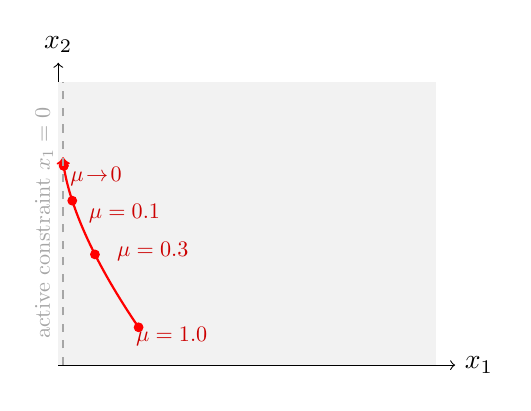
\begin{tikzpicture}[scale=1.2]
  % Axes
  \draw[->] (0,0) -- (4.2,0) node[right] {$x_1$};
  \draw[->] (0,0) -- (0,3.2) node[above] {$x_2$};
  
  % Feasible region: positive orthant
  \fill[gray!10] (0,0) rectangle (4,3);

  % % Objective contours (ellipses)
  % \foreach \a in {0.6,0.9,1.2,1.5}{
  %   \draw[gray!70] (2.5,1.5) ellipse (1.8/\a and 1.0/\a);
  % }

  % Central path approaching x1=0 boundary
  \draw[thick,red,->,domain=0:1,smooth,variable=\t]
    plot ({0.8*(1-\t)^2 + 0.05},{2.2 - 1.8*(1-\t)^1.3});

  % Points along path (decreasing mu)
  \foreach \m/\t in {1.0/0.0,0.3/0.35,0.1/0.65,0.03/0.9,0.01/0.9}{
    \filldraw[red] ({0.8*(1-\t)^2 + 0.05},{2.2 - 1.8*(1-\t)^1.3}) circle (1.3pt);
  }

  % Labels for mu values
  \node[red!80!black,scale=0.8] at (0.4,2.0) {$\mu\!\to\!0$};
  \node[red!80!black,scale=0.8] at (0.7,1.6) {$\mu=0.1$};
  \node[red!80!black,scale=0.8] at (1.0,1.2) {$\mu=0.3$};
  \node[red!80!black,scale=0.8] at (1.2,0.3) {$\mu=1.0$};

  % Optimal point on the boundary
  
  % \filldraw[blue] (0.0,2.1) circle (2pt);
  % \node[anchor=west,blue,scale=0.9] at (0.0,2.1) {$x^* = (0, x_2^*)$};

  % Annotate the active constraint line
  \draw[dashed,gray!70] (0.05,0) -- (0.05,3);
  \node[gray!70,scale=0.8,rotate=90] at (-0.15,1.5) {active constraint $x_1=0$};

\end{tikzpicture}
\end{center}


\textbf{Interpretation:}
As $\mu \downarrow 0$, $x_1(\mu) \to 0$ and the iterates approach the boundary while maintaining strict positivity, ensuring well-defined Newton steps.
\end{frame}
% Slide 4: Primal-dual IPM, residuals and convergence
\begin{frame}{Primal--dual interior-point method \& practical notes}
Primal--dual methods work with both primal and dual variables and maintain perturbed complementarity:
\[XZ e = \sigma \mu e,\quad \mu=\frac{x^T z}{n},\quad 0<\sigma\le1.
\]
A common predictor--corrector algorithm (Mehrotra) computes a predictor (affine-scaling) step, estimates a \(\sigma\), then corrects to stay close to the central path.

Key practical points:
\begin{itemize}
  \item Use sparse symmetric linear algebra to solve the Newton/KKT system efficiently.
  \item Choose step-lengths to keep iterates positive; use Mehrotra predictor-corrector for fast practical convergence.
  \item Convergence: polynomial worst-case complexity (typically 30--60 iterations for large QPs in practice).
\end{itemize}

Interior-point methods follow the central path using Newton steps on a barrier-regularized KKT system; primal--dual variants maintain both primal and dual feasibility and usually reach high accuracy in few iterations.
\end{frame}

\onput
%%% Local Variables:
%%% mode: LaTeX
%%% TeX-master: "s"
%%% End:
